\documentclass[11pt,letterpaper]{article}
\usepackage[lmargin=1in,rmargin=1in,bmargin=1in,tmargin=1in]{geometry}
\usepackage{style/quiz}
\usepackage{style/commands}

% -------------------
% Content
% -------------------
\begin{document}
\thispagestyle{title}

% Quiz 1
\quizsol \textit{True/False}: The function $f(x)= 9 - 5x$ is a linear function with slope $5$ and $y$-intercept $9$. \pspace

\sol The statement is \textit{false}. We know a function of the form $f(x)= mx + b$ is a linear function with slope $m$ and $y$-intercept $b$. Because we have $f(x)= 9 - 5x= -5x + 9$, we have $m= -5$, i.e. slope $-5$, and $y$-intercept $9$, i.e. $(0, 9)$. But then the slope is $-5$, not the given value of $5$. \pvspace{1.3cm}



% Quiz 2
\quizsol \textit{True/False}: If $f(x)= 2x - 1$ and $g(x)= 3 - x$, then $(f \circ g)(0)= f(0)g(0)= -1 \cdot 3= -3$. \pspace

\sol The statement is \textit{false}. First, note that $f(0)= 2(0) - 1= -1$, $g(0)= 3 - 0= 3$, and $f(3)= 2(3) - 1= 6 - 1= 5$. What was given was function multiplication, i.e. what was computed was $(fg)(0)= f(0) g(0)= -1 \cdot 3= -3$. What was originally written was function composition. We have $(f \circ g)(0)= f\big(g(0) \big)= f(3)= 5$. \pvspace{1.3cm}



% Quiz 3
\quizsol \textit{True/False}: Compared to the graph of $f(x)$, the graph of $5 - 3f(x + 2)$ is stretched by a factor of 3, then shifted to the right by 2 and up by 5. \pspace

\sol The statement is \textit{false}. We know that $f(x + 2)$ is the graph of $f(x)$ shifted 2 to the \textit{left}. The graph of $-3f(x + 2)$ is then the graph of $f(x)$ shifted two to the left, stretched by a factor of 3, and reflected across the $x$-axis. Finally, the graph of $5 - 3f(x + 2)$ is the graph of $f(x)$ shifted two to the left, stretched by a factor of 3, reflected across the $x$-axis, then shifted upwards by 5. \pvspace{1.3cm}



% Quiz 4
\quizsol \textit{True/False}: The function $f(x)= 4(5^{-x})$ is a concave up, decreasing, exponential function. \pspace

\sol The statement is \textit{true}. A function of the form $f(x)= Ab^x$ is an exponential function. We can summarize whether $f(x)$ is increasing or decreasing and concave up or down as follows:
        \begin{table}[!ht]
        \centering
        \begin{tabular}{cll}
        \multicolumn{1}{l}{} & \multicolumn{1}{c}{$0 < b < 1$} & \multicolumn{1}{c}{$b > 1$} \\ \cline{2-3} 
        \multicolumn{1}{c|}{$A > 0$} & \multicolumn{1}{l|}{Decreasing, Concave Up} & \multicolumn{1}{l|}{Increasing, Concave Up} \\ \cline{2-3} 
        \multicolumn{1}{c|}{$A < 0$} & \multicolumn{1}{l|}{Increasing, Concave Down} & \multicolumn{1}{l|}{Decreasing, Concave Down} \\ \cline{2-3} 
        \end{tabular}
        \end{table}	
But we have $f(x)= 4(5^{-x})= 4 (5^{-1})^x= 4 \left( \dfrac{1}{5} \right)^x$. Therefore, $f(x)$ is exponential with $A= 4 > 0$ and $0 < b= \frac{1}{5} < 1$. Therefore, $f(x)$ is a decreasing, concave up, exponential function. \pvspace{1.3cm}



% Quiz 5
\quizsol \textit{True/False}: The function $f(x)= 5(2^{1 - 2x})$ is equal to the function $g(x)= 10 \left( \dfrac{1}{4} \right)^x$. \pspace

\sol The statement is \textit{true}. Observe that we have\dots
	\[
	f(x)= 5(2^{1 - 2x})= 5 \cdot 2^1 \cdot 2^{-2x}= 10 \cdot 2^{-2x}= 10 (2^{-2})^x= 10 \left( \dfrac{1}{2^2} \right)^x= 10 \left( \dfrac{1}{4} \right)^x= g(x)
	\]



\newpage



% Quiz 6
\quizsol \textit{True/False}: $\log_5(4^{-3})= -3$ \pspace

\sol The statement is \textit{false}. Recall that $\log_b(y)$ represents the power of $b$ that yields $y$; that is, $\log_b(y)= x$ if and only if $b^x= y$. Then clearly $\log_b(b^n)= n$ because $b^n= b^n$. Notice then that in the case of $\log_b(b^n)$, the logarithmic and exponential functions `undo' each other. However, the base of the logarithm and the base of the exponential function need to match. In the case of $\log_5(4^{-3})$, $b= 5 \neq 4$ so that these do not `undo' each other. In fact, we have $\log_5(4^{-3}) \approx -2.58406$ because $5^{-2.58406} \approx 4^{-3}= \frac{1}{64}$. One case use $\log_b(b^n)= n$ in the computation of $log_5(4^{-3})= -3$ if one uses the change of base formula: $\log_b(y)= \frac{\log_a(y)}{\log_a(b)}$. In this case, we have\dots
	\[
	\log_5(4^{-3})= \dfrac{\log_4(4^{-3})}{\log_4(5)}= \dfrac{-3}{\log_4(5)} \approx \dfrac{-3}{1.160964} \approx -2.58406
	\] \pvspace{1.3cm}



% Quiz 7
\quizsol \textit{True/False}: $\ln\left( \dfrac{x^5}{\sqrt[3]{y}} \right)= 5 \ln(x) - \frac{1}{3} \ln(y)$ \pspace

\sol The statement is \textit{true}. Recall that $\log_b(x^n)= n \log_b(x)$ and $\log_b \left( \frac{x}{y} \right)= \log_b(x) - \log_b(y)$; that is, for logarithms, you can turn powers into coefficients (and vice versa) and quotients into differences (and vice versa). But then we have\dots
	\[
	\ln\left( \dfrac{x^5}{\sqrt[3]{y}} \right)= \ln\left( \dfrac{x^5}{y^{1/3}} \right)= \ln(x^5) - \ln(y^{1/3})= 5 \ln(x) - \frac{1}{3}\, \ln(y)
	\] \pvspace{1.3cm}



% Quiz 8
\quizsol \textit{True/False}: If $2^{\sqrt{x}} - 5= 3$, then $x= 9$. \pspace

\sol The statement is \textit{true}. One way of being somewhat convinced is to substitute $x= 9$:
	\[
	\left( 2^{\sqrt{x}} - 5 \right) \bigg|_{x= 9}= 2^{\sqrt{9}} - 5= 2^3 - 5= 8 - 5= 3
	\]
However, all this shows is that \textit{if} $x= 9$, then $2^{\sqrt{x}} - 5= 3$. We need to show that $2^{\sqrt{x}} - 5= 3$, then it must be the case that $x= 9$; that is, we need to solve the equation $2^{\sqrt{x}} - 5= 3$ for $x$. We have\dots
	\[
	\begin{aligned}
	2^{\sqrt{x}} - 5&= 3 \\[0.3cm]
	2^{\sqrt{x}}&= 8 \\[0.3cm]
	\log_2 \left( 2^{\sqrt{x}} \right)&= \log_2(8) \\[0.3cm]
	\sqrt{x}&= 3 \\[0.3cm]
	(\sqrt{x})^2&= 3^2 \\[0.3cm]
	x&= 9
	\end{aligned}
	\]



\newpage



% Quiz 9
\quizsol \textit{True/False}: $\tan(\theta) \cot(\theta)= 1$ \pspace

\sol The statement is \textit{true}. Recall that $\cot(\theta)= \frac{1}{\tan \theta}$. But then we have\dots
	\[
	\tan(\theta) \cot(\theta)= \tan(\theta) \cdot \dfrac{1}{\tan \theta}= 1
	\] \pvspace{1.3cm} 



% Quiz 10
\quizsol \textit{True/False}: The reference angle for the angle that is $30^\circ$ clockwise from the negative $y$-axis is $240^\circ$. \pspace

\sol The statement is \textit{false}. A reference angle is always an angle `in' Quadrant~I; that is, a reference angle $\theta$ is always such that $0 \leq \theta \leq \frac{\pi}{2}$, i.e. $0 \leq \theta \leq 90^\circ$. Therefore, it is impossible to have a reference angle of $240^\circ$. We can see in the diagram below that an angle that is $30^\circ$ clockwise from the negative $y$-axis below.
	\[
	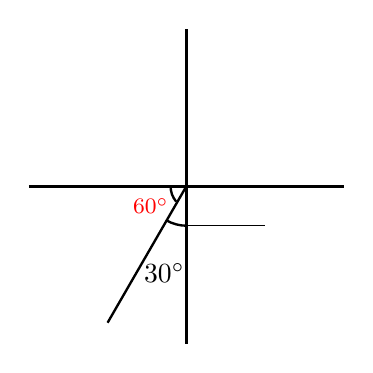
\begin{tikzpicture}
	\draw[line width=0.03cm] (-2,0) -- (2,0);
	\draw[line width=0.03cm] (0,-2) -- (0,2);
	\draw[line width=0.03cm] (0,0) -- (-1, -1.73205);
	\draw[line width=0.03cm] (0,-0.5) arc(270:240:0.5);
	\node at (-0.28,-1.1) {$30^\circ$};
	
	\draw (0,-0.5) -- (1,-0.5);
	\draw[line width=0.03cm] (-0.2,0) arc(180:220:0.3);
	\node at (-0.45,-0.25) {\footnotesize\color{red}$60^\circ$};
	\end{tikzpicture}
	\]
This is indeed an angle of $240^\circ$ with the positive $x$-axis (coming from $270^\circ - 30^\circ= 240^\circ$). However, the smallest possible angle this ray makes with the $x$-axis is $60^\circ$. Therefore, the reference angle is $60^\circ$ (represented in red in the diagram above). \pvspace{1.3cm}



% Quiz 11 
\quizsol \textit{True/False}: Because we have $\tan(\theta + 2\pi)= \tan(\theta)$ for all $\theta \in \mathbb{R}$, the period of $\tan \theta$ is $2\pi$. 

\sol The statement is \textit{false}. The period of a function $f(x)$ (if it exists) is the \textit{smallest} positive value $P$ such that $f(x + P)= f(x)$ for all $x$. While it is true that $\tan(\theta + 2\pi)= \tan(\theta)$ for all $\theta \in \mathbb{R}$, this is not necessarily the \textit{smallest} possible value such that this is true. Observe that\dots
	\[
	\tan(\theta + \pi)= \dfrac{\sin(\theta + \pi)}{\cos(\theta + \pi)}= \dfrac{-\sin(\theta)}{-\cos(\theta)}= \dfrac{\sin(\theta)}{\cos(\theta)}= \tan(\theta)
	\]
But then the period is at most $\pi$. In fact, the period of tangent is $\pi$. Therefore, $\tan(\theta + \pi)= \tan(\theta)$ for all $\theta \in \mathbb{R}$.\footnote{Note: We have only shown that the period is at most $\pi$. To show that the period is $\pi$, we need to show that there can be no smaller value, say $P$, such that $\tan(\theta + P)= \tan(\theta)$. Suppose that $\tan(\theta + P)= \tan(\theta)$. Then using the angle sum formula for tangent, we then have $\tan(\theta)= \tan(\theta + P)= \frac{\tan(\theta) + \tan(P)}{1 - \tan(\theta) \tan(P)}$. But this gives $\tan(\theta) + \tan(P)= \tan(\theta) - \tan^2(\theta) \tan(P)$. But then we have $\tan(P) \left( \tan^2(\theta) + 1 \right)= 0$. If $\tan^2(\theta) + 1= 0$, then $\left( \tan(\theta) \right)^2= -1$, which is impossible. But then it must be $\tan(P)= 0$. This implies that $P= k\pi$ for some integer $k$. The smallest (positive) solution is clearly when $k= 1$, which gives $P= \pi$.}



\newpage



% Quiz 12
\quizsol \textit{True/False}: $\cos^2(\theta)= \sin(\theta) \left( \csc(\theta) - \sin(\theta) \right)$ \pspace

\sol The statement is \textit{true}. Starting with the right hand side, we have\dots
	\[
	\begin{aligned}
	 \sin(\theta) \left( \csc(\theta) - \sin(\theta) \right)&=  \sin(\theta) \left( \dfrac{1}{\sin(\theta)} - \sin(\theta) \right) \\[0.3cm]
	 &= \dfrac{\sin(\theta)}{\sin(\theta)} - \sin^2(\theta) \\[0.3cm]
	 &= 1 - \sin^2(\theta) \\[0.3cm]
	 &= \cos^2(\theta)
	\end{aligned}
	\]
where for the last equality we have used the fact that $\sin^2(\theta) + \cos^2(\theta)= 1$, i.e. $\cos^2(\theta)= 1 - \sin^2(\theta)$. \pvspace{1.3cm}



% Quiz 13
\quizsol \textit{True/False}: There are only two solutions to the equation $\tan \theta= \sqrt{3}$. \pspace

\sol The statement is \textit{false}. We know that $\tan \left( \frac{\pi}{3} \right)= \sqrt{3}$ and $\tan \left( \frac{4\pi}{3} \right)= \sqrt{3}$. There are then at least two solutions. However, the period of $\tan(\theta)$ is $2\pi$. Then any rotation of $\frac{\pi}{3}$ by any multiple of $\pi$ radians counterclockwise or clockwise will also be a solution of the equation. For instance, all of the following are solutions to the equation $\tan(\theta)= \sqrt{3}$. 
	\[
	\begin{aligned}
	\dfrac{\pi}{3} - 2 \pi&= -\dfrac{5\pi}{3} &\qquad \dfrac{\pi}{3} + 2\pi&= \dfrac{7\pi}{3} \\[0.3cm]
	\dfrac{\pi}{3} - \pi&= -\dfrac{2\pi}{3} & \dfrac{\pi}{3} + \pi&= \dfrac{4\pi}{3}
	\end{aligned}
	\]
































\end{document}